% !TeX spellcheck = pt_BR
\documentclass[aspectratio=169, xcolor=dvipsnames]{beamer} 
%Definições de tema
\setbeamertemplate{blocks}[rounded][shadow=false]
\usetheme{Madrid}
\setbeamertemplate{items}[square]
\setbeamertemplate{caption}[numbered]
\usecolortheme{beaver}
\setbeamercolor{frametitle}{bg=white!10!white}

\usefonttheme{professionalfonts} 
\setbeamertemplate{itemize item}{\color[rgb]{0.8,0,0}$\blacksquare$}
\setbeamertemplate{itemize subitem}{\color[rgb]{0.8,0,0}$\blacksquare$}
\setbeamertemplate{itemize subsubitem}{\color[rgb]{0.8,0,0}$\blacksquare$}

%Definições de seção
\setcounter{secnumdepth}{3}
\setcounter{tocdepth}{2}


\usepackage{xkeyval}
\usepackage{todonotes}
\presetkeys{todonotes}{inline}{}


\usepackage{helvet}
\renewcommand{\familydefault}{\sfdefault}
\usepackage{float}
\usepackage[brazil]{babel}
\usepackage[utf8]{inputenc}
\usepackage{graphicx, tikz}
\usepackage{url}
\usepackage{subfigure}
\usepackage{mathtools} % setas com texto
\usepackage{multicol}
\usepackage{listings}
\usepackage{lipsum}
\usepackage{scalefnt}
\usepackage{ragged2e}
\usepackage{etoolbox, verbatim}

% Listing
\lstset{ 
	numbers=left,
	stepnumber=1,
	numbersep=6pt,
	numberstyle=\small\color{black},
	basicstyle= \scriptsize,
%	keywordstyle=\color{black},
%	commentstyle=\color{black},
%	stringstyle=\color{black},
	tabsize=2
}
%Definições Listing - Linguagem Scala
\lstdefinelanguage{scala}{
morekeywords={abstract,case,catch,class,def,%
	do,else,extends,false,final,finally,%
	for,if,implicit,import,match,mixin,%
	new,null,object,override,package,%
	private,protected,requires,return,sealed,%
	super,this,throw,trait,true,try,%
	type,val,var,while,with,yield},
otherkeywords={=>,<-,<\%,<:,>:,\#,@},
sensitive=true,
morecomment=[l]{//},
morecomment=[n]{/*}{*/},
morestring=[b]",
morestring=[b]',
morestring=[b]"""
}

\let\olditem=\item% 
\renewcommand{\item}{\olditem \justifying}

\title[Arquitetura de Computadores - RISC-V e Rocket-Chip]{\textbf{Arquitetura de Computadores}\\\textit{Reduced Instruction Set Computer: \\Estudo sobre RISC-V e Introdução ao Rocket-Chip}}
\author[\textit{rodolfolabiapari@decom.ufop.br}]{Rodolfo Labiapari Mansur Guimarães}
\institute[IFMG]{\begin{figure}
		\centering
		
\includegraphics[width=0.1\textwidth]{img/ufop.jpg}
\end{figure}}
\institute[UFOP]{
	\textit{rodolfolabiapari@decom.ufop.br} \\
	Lattes: \url{http://goo.gl/MZv4Dc} \\
	Departamento de Computação -- Universidade Federal de Ouro Preto \\
	Ouro Preto - MG -- Brasil }

\date{Última Atualização: \today}

\begin{document}


\frame{\titlepage}

\AtBeginSection[] 
{
	\begin{frame}
	\frametitle{Sumário}
	\tableofcontents[]
	\end{frame}
}

\AtBeginSubsection[] 
{
	\begin{frame}
	\frametitle{Sumário}
	\tableofcontents[
    currentsection, 
    currentsubsection, 
    hideothersubsections, 
    %sectionstyle=show/hiden, 
    subsectionstyle=show/shaded, ]
	\end{frame}
}

%\usebackgroundtemplate{
\includegraphics[trim=0cm 0cm 10cm 0cm, width=0.03\textwidth]{img/ufop.jpg}}

\section{Formato das Instruções Bases do RISC-V}
\begin{frame}{Formato das Instruções Bases}
	\begin{itemize}
		\setlength{\itemsep}{1em}
		\item Na base do ISA RISC-V, existe quatro formato de instruções principais
	\end{itemize}
	\begin{figure}
		\centering
		\label{fig:instruction-format}
		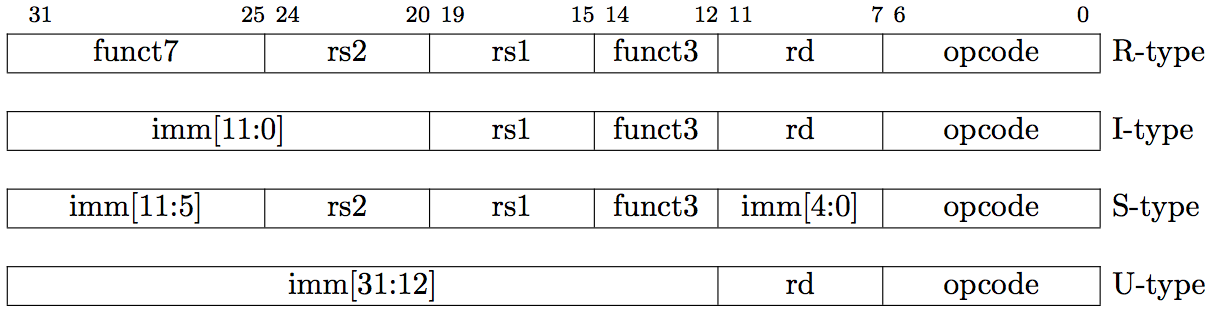
\includegraphics[width=0.8\textwidth]{img/instruction.png}
	\end{figure}
	\begin{itemize}
		\item Alguma observações
		\begin{itemize}
			\setlength{\itemsep}{0.5em}
			\item É possível ver que \textit{rd}, \textit{rs1} e \textit{rs2} estão na mesma posição
			\begin{itemize}
				\item Isso é um método para facilitação da decodificação.
			\end{itemize}
			\item Imediatos estão sempre no final da instrução;
			%\item O sinal do imediato sempre fica no bit 31.
		\end{itemize}
	\end{itemize}
\end{frame}

\subsection{RV32I}
\begin{frame}{RV32I}{Register-Immediate}
	\begin{figure}
		\centering
		\label{fig:}
		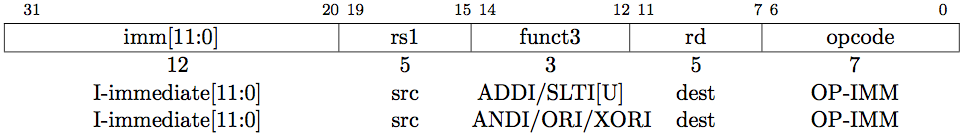
\includegraphics[width=0.9\textwidth]{img/register-immediate.png}
	\end{figure}
	\begin{itemize}
		\item \textbf{\textit{Opcode}:} Local onde fica a operação principal;
		\item \textbf{\textit{Funct3}:} Especificação da operação.
	\end{itemize}
\end{frame}

\begin{frame}{RV32I}{Register-Register}
	\begin{figure}
		\centering
		\label{fig:}
		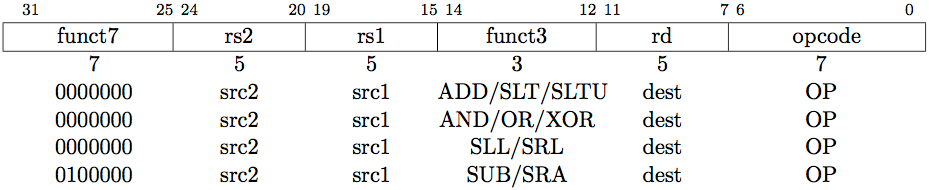
\includegraphics[width=0.9\textwidth]{img/register-register.png}
	\end{figure}
	\begin{itemize}
		\item \textbf{\textit{Opcode}:} Local onde fica a operação principal;
		\item \textbf{\textit{Funct3}:} Especificação da operação;
		\item \textbf{\textit{Funct7}:} Especificação da operação;
	\end{itemize}
\end{frame}

\begin{frame}{RV32I}{Nop}
	\begin{figure}
		\centering
		\label{fig:}
		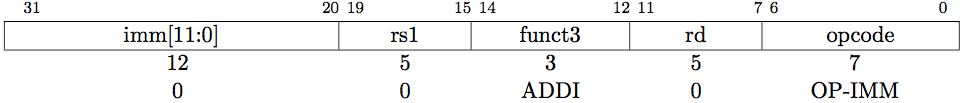
\includegraphics[width=0.9\textwidth]{img/nop.png}
	\end{figure}
\end{frame}

\begin{frame}{RV32I}{Jump and Link\footnote{\textit{Jump and Link} é um \textit{jump} com endereço de retorno.}}
	\begin{figure}
		\centering
		\label{fig:}
		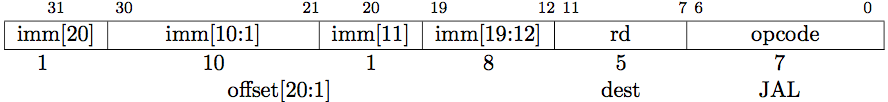
\includegraphics[width=0.9\textwidth]{img/jal.png}
	\end{figure}
\end{frame}

\begin{frame}{RV32I}{Conditional Branches}
	\begin{figure}
		\centering
		\label{fig:}
		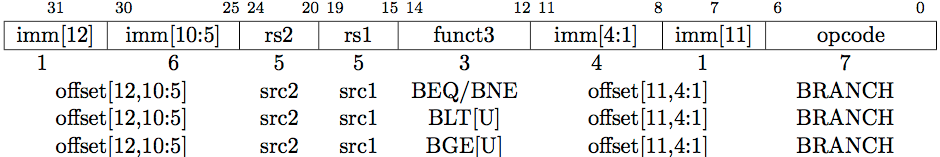
\includegraphics[width=0.9\textwidth]{img/conditional-branch.png}
	\end{figure}
\end{frame}

\begin{frame}{RV32I}{Load e Store}
	\begin{figure}
		\centering
		\label{fig:}
		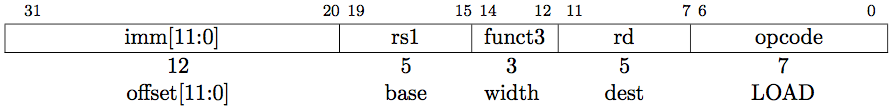
\includegraphics[width=0.9\textwidth]{img/load.png}\\[1cm]
		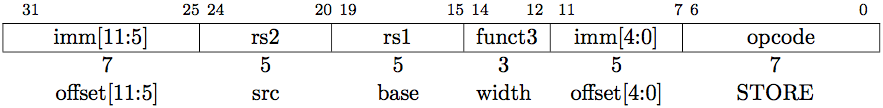
\includegraphics[width=0.9\textwidth]{img/store.png}
	\end{figure}
\end{frame}

\subsection{Comparação de Instruções entre diferentes Arquiteturas e Expansões}
\begin{frame}{RV32I vs. RV64I vs. Extensão C (compacta)}{Register-Immediate}
	\begin{figure}
		\centering
		\label{fig:}
		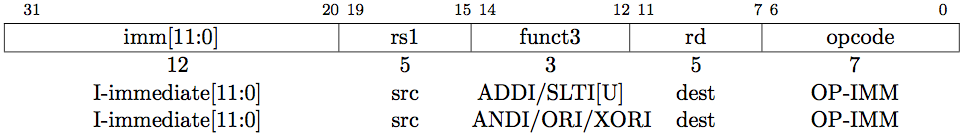
\includegraphics[width=0.9\textwidth]{img/register-immediate.png}\\[0.5cm]
		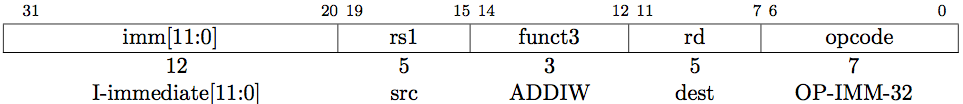
\includegraphics[width=0.9\textwidth]{img/register-immediate-64.png}\\[0.5cm]
		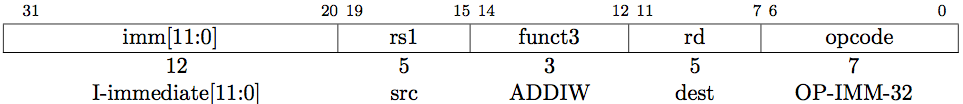
\includegraphics[width=0.9\textwidth]{img/register-immediate-64.png}
	\end{figure}
\end{frame}

\begin{frame}{RV32I vs. Extensão F}{Load e Store}
	\begin{figure}
		\centering
		\label{fig:}
		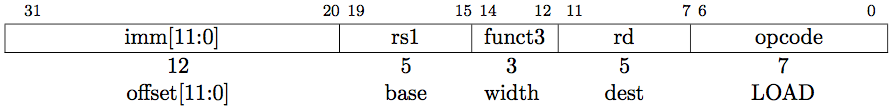
\includegraphics[width=0.8\textwidth]{img/load.png}\\
		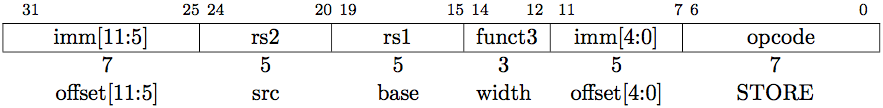
\includegraphics[width=0.8\textwidth]{img/store.png}\\[0.8cm]
		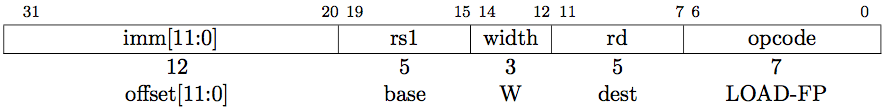
\includegraphics[width=0.8\textwidth]{img/load-pf.png}\\
		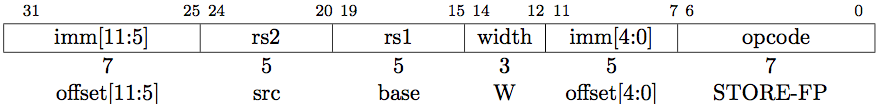
\includegraphics[width=0.8\textwidth]{img/store-pf.png}
	\end{figure}
\end{frame}

\begin{comment}
muito pequeno pro projetor
\section{Datapath do Projeto}
{
\setbeamertemplate{navigation symbols}{}
\begin{frame}[plain]
\begin{figure}
\centering
\label{fig:}
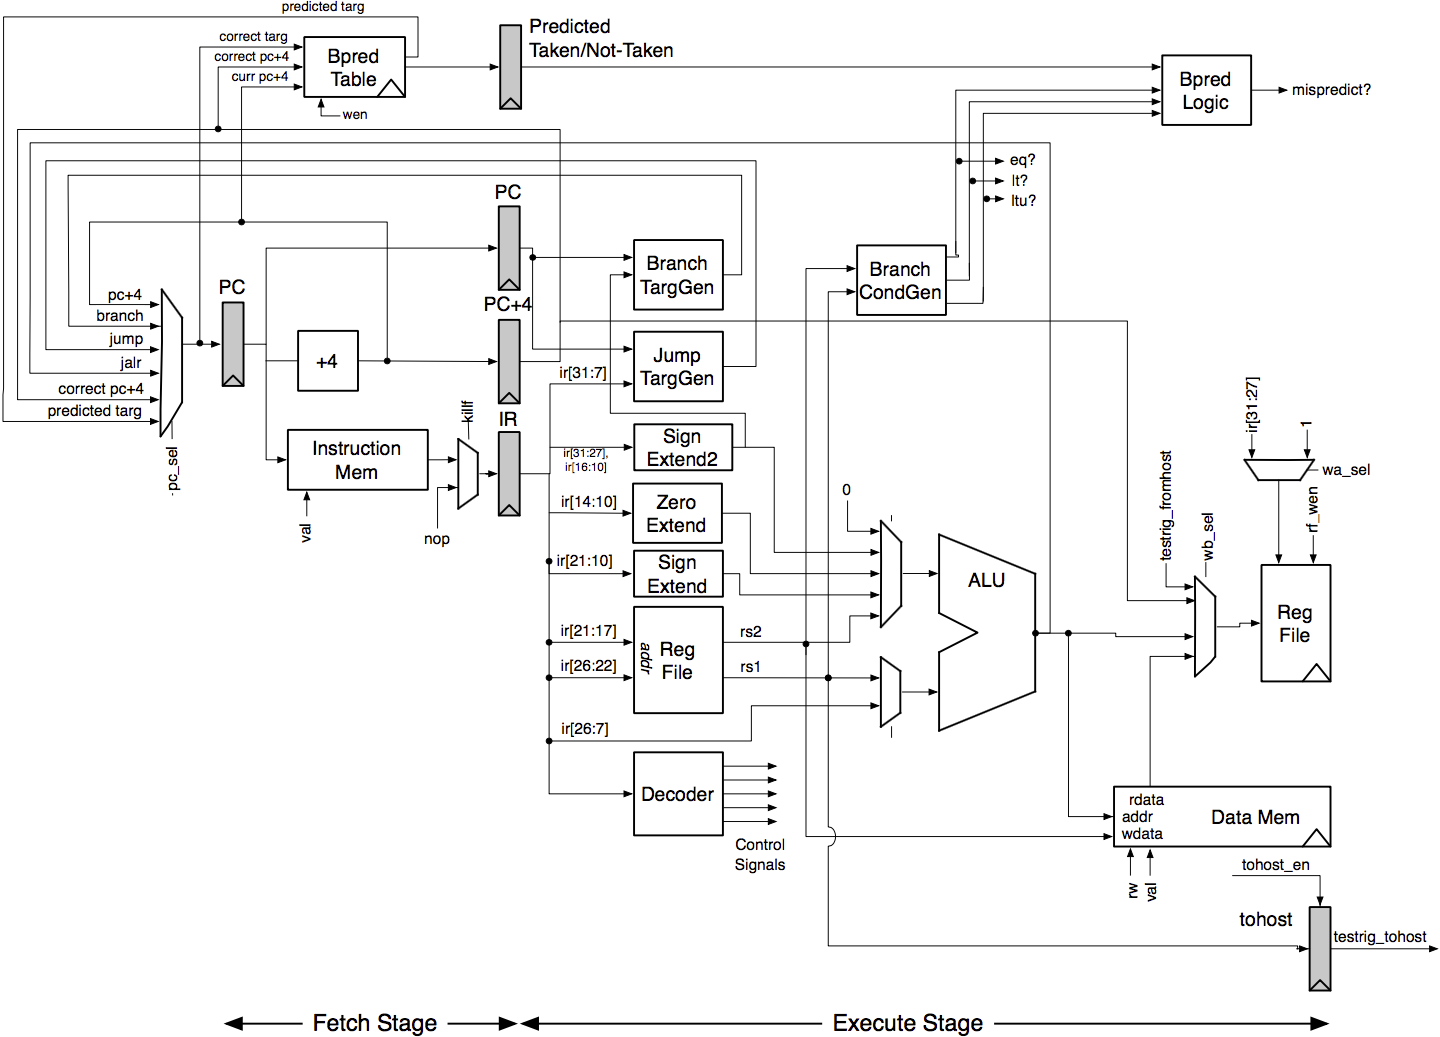
\includegraphics[width=0.795\textwidth]{img/two-stages.png}
\end{figure}
\end{frame}
}

\end{comment}

\section{Tutorial RISC-V Rocket Chip}
\begin{frame}{Rocket Chip}{Introdução}
	\begin{itemize}
		\setlength{\itemsep}{1.5em}
		\item Rocket Chip permite gerar diferentes configurações de SoC\footnote{\textit{System-on-a-chip:} se refere a todos os componentes de um computador/sistema eletrônico, em um circuito integrado.}.
	
		\item Essas configurações são especificadas por meio de parâmetros em linguagem Chisel\footnote{\textit{Constructing Hardware In a Scala Embedded Language}.} que podem ser alterados livremente:
		\begin{itemize}
			\item E com isso, pode-se selecionar o que quer gerar como chip.
		\end{itemize}
		\item Também possui um emulador C++ de RLT\footnote{\textit{Register transfer level}.}.
	\end{itemize}
\end{frame}

\begin{frame}{Rocket Chip}{Introdução}
	\begin{itemize}
		\setlength{\itemsep}{1.5em}
		\item Rocket Chip é formado por vários submódulos:
		\begin{itemize}
			\setlength{\itemsep}{0.8em}
			\item \textbf{Chisel}: Linguagem HDL para desenvolvimento de RTL;
			\item \textbf{Rocket}: Código-fonte dos \textit{cores} e \textit{caches} do Rocket;
			\item \textbf{Dramsim2}: Simulador de tempos de acesso à DRAM; 
			\item Entre outros.
		\end{itemize}
	
		\item Algumas configurações possíveis:
		\begin{itemize}
			\setlength{\itemsep}{0.8em}
			\item Quantidade memória física;
			\item Quantidade de bits do endereço virtual;
			\item Parâmetros de interface de memória;
			\item E outros.
		\end{itemize}
	\end{itemize}
\end{frame}

\begin{frame}{Rocket Chip}{Simulando uma Configuração Predefinida}
	\begin{itemize}
		\setlength{\itemsep}{1.5em}
		\item Para uma simulação, deve-se ir ao respectivo diretório.
		
		\item O emulador C++ RTL é executado do diretório \texttt{/emulator}.
		
		\item Neste diretório, um comando de execução \textit{default} já é conhecido para verificar se a ferramenta foi instalada com sucesso. Possui a seguinte sintaxe \\\texttt{make run-asm-tests} .
		
		\item Podemos também construir itens com configurações de pequeno porte utilizando a especificação  \texttt{CONFIG=ExampleSmallConfig} 
		\begin{itemize}
			\item E para testar, utiliza-se \\\texttt{make CONFIG=ExampleSmallConfig run-asm-tests} .
		\end{itemize}
	\end{itemize}
\end{frame}
\begin{comment}
Chato
\begin{frame}[fragile]{Rocket Chip}{Simulando uma Nova Configuração}
	\begin{itemize}
		\setlength{\itemsep}{0.7em}
		\item Vamos alterar o \textit{default} para uma configuração de médio porte
		\begin{itemize}
			\item \textit{``Queremos o dobro de números de caminhos em caches L1 Instruction e Data sobre uma configuração de pequeno porte''}
			
			\begin{lstlisting}[language=Scala]
				class MediumConfig extends SmallConfig{
				    override val knobValues:Any=>Any = {
				        case "L1D_WAYS" => 2
				        case "L1I_WAYS" => 2
				    }
				}
				class ExampleMediumConfig extends ChiselConfig(
				    new MediumConfig ++ new DefaultConfig)
			\end{lstlisting}
		\end{itemize}
		\item Para configurar depois testar, basta \\\texttt{make CONFIG=ExampleMediumConfig}
		\\\texttt{make CONFIG=ExampleMediumConfig run-asm-tests}
	\end{itemize}
\end{frame}

\begin{frame}{Rocket Chip}{Linguagem HDL: Verilog para CADs}
	\begin{itemize}
		\setlength{\itemsep}{0.5em}
		\item O diretório \texttt{/vsim} contém \textit{scripts} construtores que geram código em Verilog.
		
		\item Para gerar o código Verilog do projeto, basta utilizar o comando de geração \\\texttt{make} .
		
		\item O diretório do código gerado contém
		\begin{itemize}
			\item Códigos em Verilog;
			\item Conjunto de parâmetros exportados;
			\item Parâmetros de configuração de memória.
		\end{itemize}
	
		\item Os parâmetros de configuração de memória são usados em nosso projeto para descobrir qual memória SRAM será requisitada ou gerada.
		
			\bigskip
			
		\item Depois deste processo, o código em Verilog está pronto para ser utilizado em ferramentas CAD\footnote{Computer Aided Design.} como simuladores.
	\end{itemize}
\end{frame}

\begin{frame}{Rocket Chip}{Linguagem HDL: Verilog para FPGA}
	\begin{itemize}
		\setlength{\itemsep}{1.5em}
		\item Da mesma forma que o diretório anterior (\texttt{/vsim}) era utilizado para geração de código de ferramentas CAD, existe outro para geração de código especificamente para \textit{hardware} reconfiguráveis como o FPGA.
		
		\item Este diretório encontra-se em \texttt{/fsim} e para gerar os códigos, basta utilizar o \texttt{make} como anteriormente.
		
		\item Ele também gera tipicamente os mesmos arquivos que da execução anterior.
		
		\item E o código gerado está pronto para ser adaptado à placa a ser sintetizado.
	\end{itemize}
\end{frame}

\end{comment}


\begin{frame}{Dúvidas, Sugestões ou Reclamações?}
	\begin{itemize}
		\item \url{rodolfolabiapari@decom.ufop.br} \\[1cm]
		\item \url{https://www.guerrillamail.com/}
	\end{itemize}
\end{frame}

\frame{\titlepage}


\end{document}